\section[From Convolutions to Graphs: The CNN-GNN Connection]{From Convolutions to Graphs: The \glspl{CNN}-\glspl{GNN} Connection}\label{sec:cnn_as_gnn}

\subsection{Preliminaries: Graph Theory}\label{subsec:preliminares_grafos_cnn}

For the basic definition of a graph, see \autoref{def:grafo_neuronal} in \autoref{ch:neural_networks}. In this section we focus on its specific relationship with convolutions.

\begin{definition}[Representation of Data as Graphs]\label{def:representacion_datos_grafos}
Data is represented in a graph by means of:
\begin{itemize}
	\item \textbf{Node features}: \(X \in \mathbb{R}^{n \times d}\) where \(x_i \in \mathbb{R}^d\) is the feature of node \(i\)
	\item \textbf{Adjacency matrix}: \(A \in \{0,1\}^{n \times n}\) where \(A_{ij} = 1\) if \((v_i, v_j) \in E\)
	\item \textbf{Edge features} (optional): \(E \in \mathbb{R}^{|E| \times d_e}\)
\end{itemize}
\end{definition}

\begin{example}[Different Types of Data as Graphs]
\leavevmode
\begin{enumerate}
	\item \textbf{Molecules}: atoms = nodes, bonds = edges
	\item \textbf{Social networks}: people = nodes, relationships = edges
	\item \textbf{Images}: pixels = nodes, neighborhood = edges (special case!)
	\item \textbf{Point clouds}: points = nodes, k-NN = edges
\end{enumerate}
\end{example}

\begin{figure}[htbp]
	\centering
	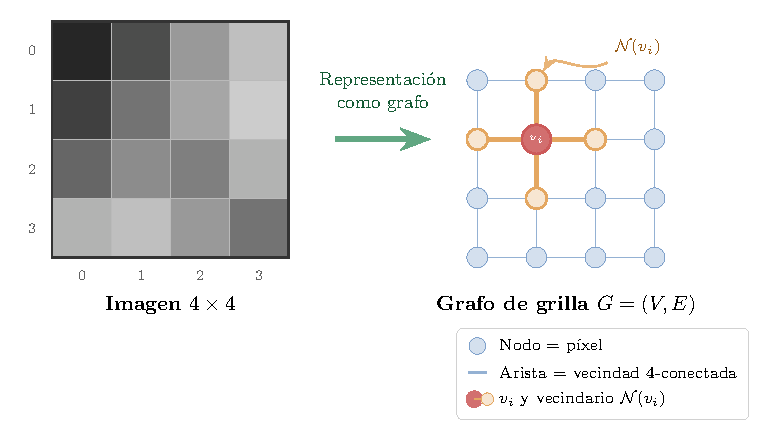
\includegraphics[width=0.85\textwidth]{images/image_as_graph}
	\caption[Image as a regular grid graph]{An image can be represented as a regular grid graph with 4-connectivity: each pixel is a node and the edges connect horizontally and vertically neighboring pixels. The neighborhood $\mathcal{N}(v_i)$ corresponds exactly to the support of the convolutional kernel.}
	\label{fig:image_as_graph}
\end{figure}

\begin{example}[Explicit Construction: 3×3 Image as a Graph]\label{ex:imagen_3x3_grafo}
Consider an RGB image of size $3 \times 3$ with 3 color channels. The transformation into a graph proceeds in three steps:

\textbf{Step 1: Node identification}. Each pixel $(i,j)$ is mapped to a node $v_{i,j}$ of the graph:
\[
V = \{v_{0,0}, v_{0,1}, v_{0,2}, v_{1,0}, v_{1,1}, v_{1,2}, v_{2,0}, v_{2,1}, v_{2,2}\}
\]
with $|V| = 9$ nodes.

\textbf{Step 2: Edge construction}. For 4-connectivity, we connect horizontally and vertically adjacent pixels:
\begin{align}
E = \{&(v_{0,0}, v_{0,1}), (v_{0,1}, v_{0,2}), \quad \text{(row 0)} \\
    &(v_{1,0}, v_{1,1}), (v_{1,1}, v_{1,2}), \quad \text{(row 1)} \\
    &(v_{2,0}, v_{2,1}), (v_{2,1}, v_{2,2}), \quad \text{(row 2)} \\
    &(v_{0,0}, v_{1,0}), (v_{1,0}, v_{2,0}), \quad \text{(column 0)} \\
    &(v_{0,1}, v_{1,1}), (v_{1,1}, v_{2,1}), \quad \text{(column 1)} \\
    &(v_{0,2}, v_{1,2}), (v_{1,2}, v_{2,2}) \} \quad \text{(column 2)}
\end{align}
We obtain $|E| = 12$ undirected edges.

\textbf{Step 3: Feature assignment}. Each node $v_{i,j}$ receives a feature vector $\mathbf{x}_{i,j} \in \mathbb{R}^3$ corresponding to the RGB values of pixel $(i,j)$:
\[
X = \begin{bmatrix} \mathbf{x}_{0,0}^T \\ \mathbf{x}_{0,1}^T \\ \vdots \\ \mathbf{x}_{2,2}^T \end{bmatrix} \in \mathbb{R}^{9 \times 3}
\]

The adjacency matrix $A \in \{0,1\}^{9 \times 9}$ has the block-tridiagonal form characteristic of regular grids.
\end{example}

\textbf{Special Properties of Grid Graphs.} Grid graphs derived from images possess unique structural properties:
\begin{enumerate}
    \item \textbf{Regularity}: Nearly constant degree ($\deg(v) = 4$ except at borders)
    \item \textbf{Spatial structure}: Positions $(i,j)$ define a natural embedding in $\mathbb{R}^2$
    \item \textbf{Symmetry}: Invariance to discrete translations
    \item \textbf{Predictable spectrum}: The eigenvalues of the Laplacian are known analytically
\end{enumerate}

These properties make CNNs especially effective on grids, but they also limit their applicability to general graphs.

\subsection[CNNs as GNNs on Regular Grids]{\glspl{CNN} as \glspl{GNN} on Regular Grids}\label{subsec:cnns_como_gnns_grillas}

\begin{theorem}[A \gls{CNN} is a Special Case of a \gls{GNN}]\label{thm:cnn_caso_especial_gnn}
A 2D \gls{CNN} is exactly equivalent to a \gls{GNN} where:
\begin{itemize}
	\item \textbf{Graph}: Regular grid \(G = (\mathbb{Z}^2 \cap \Omega, E)\)
	\item \textbf{Vertices}: Pixels at positions \((i,j)\)
	\item \textbf{Edges}: 4- or 8-neighbor connectivity
	\item \textbf{Weights}: Shared according to relative position (kernel)
\end{itemize}
\end{theorem}

\begin{proof}
The equivalence is established through the natural correspondence:
\begin{enumerate}
	\item Each pixel \((i,j)\) corresponds to a node \(v_{i,j}\) in the graph
	\item The spatial connections define the edges: \((v_{i,j}, v_{i',j'}) \in E\) if and only if \(|i-i'| + |j-j'| \leq 1\)
	\item The convolutional kernel \(K\) determines the edge weights according to the relative distance
	\item The aggregation operation in \glspl{GNN} reduces exactly to 2D convolution
\end{enumerate}
\end{proof}

\begin{definition}[Grid as a Graph]\label{def:grilla_como_grafo}
For an image of size \(H \times W\):
\begin{itemize}
	\item \(V = \{(i,j) : 0 \leq i < H, 0 \leq j < W\}\)
	\item \(E = \{((i,j), (i',j')) : |i-i'| + |j-j'| \leq 1\}\) (4-connectivity)
	\item Constant degree: \(\deg(v) = 4\) (except at borders)
\end{itemize}
\end{definition}

\begin{theorem}[Constructive CNN-GNN Equivalence]\label{thm:equivalencia_constructiva_cnn_gnn}
Given a CNN with an architecture of convolutional layers $\{L_\ell\}_{\ell=1}^L$ operating on $H \times W$ grids, there exists an explicit construction of an equivalent GNN that produces identical outputs for every input.

\textbf{Construction}:
\begin{enumerate}
    \item \textbf{Graph}: $G = (V, E)$ where $V = \{(i,j) : 0 \leq i < H, 0 \leq j < W\}$ and
    \[
    E = \{((i,j), (i',j')) : |i-i'| + |j-j'| = 1\}
    \]

    \item \textbf{Initial features}: For each node $v_{i,j}$, assign $h_{v_{i,j}}^{(0)} = x_{i,j}$ where $x_{i,j}$ is the pixel value at $(i,j)$

    \item \textbf{Message function}: For a CNN kernel $K \in \mathbb{R}^{k \times k \times c_{\text{in}} \times c_{\text{out}}}$, define
    \[
    M_\ell(h_v^{(\ell)}, h_u^{(\ell)}, e_{vu}) = W_{v-u}^{(\ell)} h_u^{(\ell)}
    \]
    where $W_{v-u}^{(\ell)} \in \mathbb{R}^{c_{\text{out}} \times c_{\text{in}}}$ is the submatrix of the kernel corresponding to the displacement $(v-u)$

    \item \textbf{Aggregation}:
    \[
    m_v^{(\ell+1)} = \sum_{u \in \mathcal{N}(v)} M_\ell(h_v^{(\ell)}, h_u^{(\ell)}, e_{vu})
    \]

    \item \textbf{Update}:
    \[
    h_v^{(\ell+1)} = \sigma(m_v^{(\ell+1)} + b^{(\ell)})
    \]
    where $\sigma$ is the activation function and $b^{(\ell)}$ the bias
\end{enumerate}

This construction guarantees that $h_v^{(\ell)} = y_{i,j}^{(\ell)}$ for every node $v = (i,j)$ and layer $\ell$, where $y_{i,j}^{(\ell)}$ is the CNN activation at position $(i,j)$ of layer $\ell$.
\end{theorem}

\begin{proof}
We proceed by induction on the depth of the network.

\textbf{Base case} ($\ell = 0$): By construction, $h_v^{(0)} = x_{i,j} = y_{i,j}^{(0)}$ for every node $v = (i,j)$.

\textbf{Inductive step}: Suppose $h_v^{(\ell)} = y_{i,j}^{(\ell)}$ for every $v = (i,j)$. We must show that $h_v^{(\ell+1)} = y_{i,j}^{(\ell+1)}$.

For the CNN, the output at position $(i,j)$ of layer $\ell+1$ is:
\begin{align}
y_{i,j}^{(\ell+1)} &= \sigma\left(\sum_{(u,v) \in \mathcal{K}} K_{u,v} \cdot x_{i+u,j+v}^{(\ell)} + b^{(\ell)}\right) \\
&= \sigma\left(\sum_{(i',j') \in \mathcal{N}(i,j)} K_{i'-i,j'-j} \cdot y_{i',j'}^{(\ell)} + b^{(\ell)}\right)
\end{align}

where $\mathcal{K}$ is the support of the kernel and $\mathcal{N}(i,j)$ the neighborhood of pixel $(i,j)$.

For the GNN, using the proposed construction:
\begin{align}
h_v^{(\ell+1)} &= \sigma\left(\sum_{u \in \mathcal{N}(v)} W_{v-u}^{(\ell)} h_u^{(\ell)} + b^{(\ell)}\right) \\
&= \sigma\left(\sum_{(i',j') \in \mathcal{N}(i,j)} K_{i'-i,j'-j} \cdot h_{(i',j')}^{(\ell)} + b^{(\ell)}\right) \\
&\overset{\text{I.H.}}{=} \sigma\left(\sum_{(i',j') \in \mathcal{N}(i,j)} K_{i'-i,j'-j} \cdot y_{i',j'}^{(\ell)} + b^{(\ell)}\right) \\
&= y_{i,j}^{(\ell+1)}
\end{align}

where we used the inductive hypothesis (I.H.) in the third equality. $\square$
\end{proof}

\begin{example}[Numerical Verification: 3×3 Sobel Kernel]\label{ex:verificacion_numerica_sobel}
Consider the horizontal Sobel kernel:
\[
K = \begin{bmatrix} -1 & 0 & 1 \\ -2 & 0 & 2 \\ -1 & 0 & 1 \end{bmatrix}
\]

Applied to the $3 \times 3$ image:
\[
I = \begin{bmatrix} 0 & 1 & 2 \\ 0 & 1 & 2 \\ 0 & 1 & 2 \end{bmatrix}
\]

\textbf{CNN method}: The convolution at the central pixel $(1,1)$ produces:
\begin{align}
y_{1,1} &= -1 \cdot 0 + 0 \cdot 1 + 1 \cdot 2 \\
        &\quad + (-2) \cdot 0 + 0 \cdot 1 + 2 \cdot 2 \\
        &\quad + (-1) \cdot 0 + 0 \cdot 1 + 1 \cdot 2 \\
        &= 0 + 2 + 0 + 4 + 0 + 2 = 8
\end{align}

\textbf{GNN method}: We construct the graph with $v_{1,1}$ connected to its 8 neighbors. The messages are:
\begin{align}
m_{1,1} &= K_{-1,-1} \cdot h_{0,0} + K_{-1,0} \cdot h_{0,1} + K_{-1,1} \cdot h_{0,2} \\
        &\quad + K_{0,-1} \cdot h_{1,0} + K_{0,1} \cdot h_{1,2} \\
        &\quad + K_{1,-1} \cdot h_{2,0} + K_{1,0} \cdot h_{2,1} + K_{1,1} \cdot h_{2,2} \\
        &= (-1)(0) + (0)(1) + (1)(2) + (-2)(0) + (2)(2) \\
        &\quad + (-1)(0) + (0)(1) + (1)(2) = 8
\end{align}

Both methods produce the identical result $y_{1,1} = 8$, verifying the equivalence.
\end{example}

\subsection{Convolution-Message Passing Equivalence}\label{subsec:equivalencia_conv_mp}

\begin{theorem}[Fundamental Equivalence]\label{thm:equivalencia_fundamental_conv_mp}
The 2D convolution operation:
\[
y_{i,j} = \sum_{(u,v) \in \mathcal{N}} K_{u,v} \cdot x_{i+u,j+v}
\]

is exactly equivalent to message passing on the grid:
\[
m_{(i,j)} = \sum_{(i',j') \in N(i,j)} K_{i'-i,j'-j} \cdot x_{i',j'}
\]

where \(N(i,j)\) are the neighbors of pixel \((i,j)\).
\end{theorem}

\begin{proof}
The convolution sums over a fixed neighborhood relative to the central pixel.
On the regular grid, this neighborhood corresponds exactly to the
neighbors in the graph with weights determined by the relative position.
The kernel weights \(K_{u,v}\) correspond to the weighted messages. \(\square\)
\end{proof}

\begin{figure}[htbp]
	\centering
	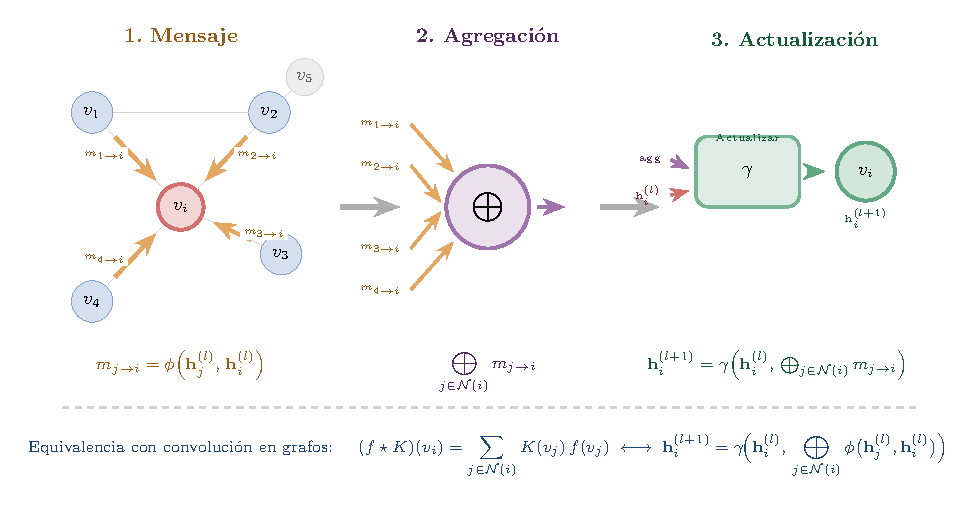
\includegraphics[width=0.90\textwidth]{images/conv_message_passing}
	\caption[Convolution-message passing equivalence]{Equivalence between convolution and message passing: the three fundamental steps (message, aggregation, update) correspond exactly to the convolutional operation when the graph is a regular grid.}
	\label{fig:conv_message_passing}
\end{figure}

\begin{example}[Step-by-Step Demonstration: Convolution = Message Passing]\label{ex:paso_a_paso_conv_mp}
Consider a 1D signal $f = [1, 3, 2, 4]$ and a kernel $K = [0.5, 1, 0.5]$ (smoothing filter).

\textbf{Interpretation as convolution}:
\begin{align}
(f * K)[1] &= 0.5 \cdot f[0] + 1 \cdot f[1] + 0.5 \cdot f[2] \\
           &= 0.5 \cdot 1 + 1 \cdot 3 + 0.5 \cdot 2 = 4.5
\end{align}

\textbf{Interpretation as message passing}:
We construct a linear graph $v_0 \leftrightarrow v_1 \leftrightarrow v_2 \leftrightarrow v_3$ with initial features $h_{v_i}^{(0)} = f[i]$.

The messages received by node $v_1$ are:
\begin{itemize}
    \item From $v_0$: $m_{v_1 \leftarrow v_0} = W_{-1} \cdot h_{v_0}^{(0)} = 0.5 \cdot 1 = 0.5$
    \item Self-message: $m_{v_1 \leftarrow v_1} = W_0 \cdot h_{v_1}^{(0)} = 1 \cdot 3 = 3$
    \item From $v_2$: $m_{v_1 \leftarrow v_2} = W_{+1} \cdot h_{v_2}^{(0)} = 0.5 \cdot 2 = 1$
\end{itemize}

Aggregation produces:
\[
m_{v_1}^{(1)} = \sum_{u \in \mathcal{N}(v_1)} m_{v_1 \leftarrow u} = 0.5 + 3 + 1 = 4.5
\]

Once again, both approaches produce the same result: $4.5$.
\end{example}

\textbf{Connection with the Unified MPNN Framework.} The convolution-message passing equivalence established in this section is a special case of the \textit{Message Passing Neural Networks} (\glspl{MPNN}) framework introduced in \autoref{def:mpnn_unificador} of \autoref{ch:gdl}.

Specifically, CNNs correspond to MPNNs with:
\begin{itemize}
    \item \textbf{Fixed graph}: Regular grid with local connectivity
    \item \textbf{Message function}: $M_\ell(h_v, h_u, e_{vu}) = W_{v-u}^{(\ell)} h_u$ (dependence only on the relative displacement)
    \item \textbf{Aggregation}: Unweighted sum $m_v = \sum_{u \in \mathcal{N}(v)} M_\ell(\cdot)$
    \item \textbf{Update}: $U_\ell(h_v, m_v) = \sigma(m_v + b^{(\ell)})$
\end{itemize}

This formulation reveals that the fundamental restriction of CNNs is \textbf{weight sharing based on relative position} ($W_{v-u}$), which only makes sense in domains with a translation structure. For general graphs lacking such structure, we need more flexible message functions, as explored in \autoref{subsec:message_passing_unificador} of \autoref{ch:gdl}.

\begin{proposition}[Computational Complexity of CNN vs GNN on Grids]\label{prop:complejidad_cnn_vs_gnn_grilla}
For an image of size $H \times W$ with $C$ channels and a $k \times k$ kernel:
\begin{itemize}
    \item \textbf{Standard CNN}: $O(H \cdot W \cdot k^2 \cdot C)$ operations
    \item \textbf{GNN on a grid}: $O(|E| \cdot C) = O(4HW \cdot C)$ operations (for 4-connectivity)
\end{itemize}

When $k$ is small (typically $k \in \{3, 5, 7\}$), both complexities are equivalent: $O(HWC)$. However, the GNN formulation reveals that the complexity fundamentally depends on the number of edges $|E|$, not on the kernel size, providing a unified perspective for analyzing efficiency across different graph topologies.
\end{proposition}

\begin{proof}
\textbf{Standard CNN}: The image has $H \cdot W$ spatial positions. At each position, the $k \times k$ kernel performs $k^2$ multiplications over each of the $C$ channels, giving a total of $O(H \cdot W \cdot k^2 \cdot C)$ operations.

\textbf{GNN on a grid}: Each node (pixel) has at most 4 neighbors in 4-connectivity (up, down, left, right), so $|E| = O(4HW)$. The message passing step processes $C$ channels per edge, resulting in $O(4HW \cdot C) = O(|E| \cdot C)$ operations.
\end{proof}

\textbf{Dual Perspective: Spatial vs. Spectral.} The equivalence established in this section admits two complementary interpretations:

\textbf{Spatial perspective}: The convolution aggregates information from local neighbors with shared weights determined by the relative position. This is the natural formulation of CNNs.

\textbf{Spectral perspective}: As developed in \autoref{sec:analisis_armonico}, the convolution corresponds to multiplication in the Fourier domain. For regular grids, the eigenvectors of the Laplacian are exactly the discrete Fourier bases, establishing the connection with \autoref{def:convolucion_espectral_grafos}.

This spatial-spectral duality is fundamental: classical CNNs operate in the spatial domain for computational efficiency, while spectral formulations provide the theoretical tools to generalize to arbitrary graphs through the Chebyshev approximation (\autoref{ex:chebyshev_aproximacion}).

\subsection{Grid Laplacian and Filters}\label{subsec:laplaciano_grilla_filtros}

\begin{definition}[Discrete Laplacian on a 2D Grid]\label{def:laplaciano_discreto_grilla}
The Laplacian operator on a grid:
\[
\mathcal{L} = D - A
\]
where \(D\) is the degree matrix and \(A\) the adjacency matrix.

For a 2D grid with 4-connectivity:
\begin{align}
\mathcal{L}_{(i,j),(i,j)} &= 4 \\
\mathcal{L}_{(i,j),(i \pm 1,j)} = \mathcal{L}_{(i,j),(i,j \pm 1)} &= -1
\end{align}
\end{definition}

\begin{example}[Laplacian Kernel as a CNN Filter]
The discrete Laplacian corresponds to the kernel:
\[
K = \begin{bmatrix}
 0 & -1 &  0 \\
-1 &  4 & -1 \\
 0 & -1 &  0
\end{bmatrix}
\]
This is a classical edge detector in image processing, and its spectral interpretation as a high-pass filter is formalized in \autoref{thm:cnns_filtros_espectrales_grillas}.
\end{example}

\begin{proposition}[Eigenvalues of the Laplacian on a Rectangular Grid]\label{prop:eigenvalores_laplaciano_grilla}
For a 2D grid of size $n_1 \times n_2$ with periodic boundary conditions, the eigenvalues of the Laplacian are:
\begin{equation}
\lambda_{k_1,k_2} = 4 - 2\cos\!\left(\frac{2\pi k_1}{n_1}\right) - 2\cos\!\left(\frac{2\pi k_2}{n_2}\right), \quad 0 \leq k_i < n_i
\end{equation}
with eigenvectors $\phi_{k_1,k_2}(i,j) = \frac{1}{\sqrt{n_1 n_2}} e^{2\pi \imath(k_1 i/n_1 + k_2 j/n_2)}$, which are exactly the discrete Fourier bases.
\end{proposition}

\begin{proof}
For periodic boundary conditions, the functions $\phi_{k_1,k_2}$ satisfy $\phi_{k_1,k_2}(i + n_1, j) = \phi_{k_1,k_2}(i,j)$. Applying the Laplacian:
\begin{align}
(\mathcal{L}\phi_{k_1,k_2})(i,j) &= 4\phi_{k_1,k_2}(i,j) - \phi_{k_1,k_2}(i+1,j) - \phi_{k_1,k_2}(i-1,j) - \phi_{k_1,k_2}(i,j+1) - \phi_{k_1,k_2}(i,j-1) \\
&= \left(4 - e^{2\pi \imath k_1/n_1} - e^{-2\pi \imath k_1/n_1} - e^{2\pi \imath k_2/n_2} - e^{-2\pi \imath k_2/n_2}\right)\phi_{k_1,k_2}(i,j) \\
&= \left(4 - 2\cos\!\left(\frac{2\pi k_1}{n_1}\right) - 2\cos\!\left(\frac{2\pi k_2}{n_2}\right)\right)\phi_{k_1,k_2}(i,j)
\end{align}
confirming that $\phi_{k_1,k_2}$ is an eigenvector with eigenvalue $\lambda_{k_1,k_2}$.
\end{proof}

\begin{remark}[Frequency Interpretation of the Eigenvalues]\label{rem:interpretacion_frecuencial_eigenvalores}
The eigenvalues of the Laplacian on the grid admit a direct frequency interpretation:
\begin{itemize}
    \item \textbf{Zero frequency}: $\lambda_{0,0} = 0$ corresponds to the DC component (constant signal); the eigenvector $\phi_{0,0} = 1/\sqrt{n_1 n_2}$ is uniform.
    \item \textbf{Low frequencies}: small eigenvalues ($k_1, k_2$ close to 0) correspond to smooth variations on the grid. A low-pass filter selects these modes.
    \item \textbf{High frequencies}: large eigenvalues (close to $\lambda_{\max} = 8$ for the square grid) correspond to rapid variations. A high-pass filter (such as the Laplacian) selects these modes.
    \item \textbf{Maximum frequency}: $\lambda_{n/2,n/2} = 8$ corresponds to the maximum possible oscillation (checkerboard pattern $(-1)^{i+j}$).
\end{itemize}
\end{remark}

\begin{example}[Low-Pass and High-Pass Filters on the Grid]\label{ex:filtros_paso_bajo_alto}
Classical image-processing filters have precise spectral interpretations:

\textbf{Smoothing filter ($3 \times 3$ mean)}: The kernel $K_{\text{media}} = \frac{1}{9}\begin{bsmallmatrix} 1 & 1 & 1 \\ 1 & 1 & 1 \\ 1 & 1 & 1 \end{bsmallmatrix}$ acts as a low-pass filter, attenuating the high-frequency components (large eigenvalues of the Laplacian) while preserving the low-frequency components.

\textbf{Sharpening filter}: The kernel $K_{\text{sharp}} = \begin{bsmallmatrix} 0 & -1 & 0 \\ -1 & 5 & -1 \\ 0 & -1 & 0 \end{bsmallmatrix} = I + \mathcal{L}$ amplifies the high-frequency components, where $I$ preserves the original signal and $\mathcal{L}$ adds the local differences.

In the spectral domain, the response of these filters is:
\begin{align}
\hat{K}_{\text{media}}(\lambda) &\approx 1 - c\lambda + O(\lambda^2) \quad \text{(low-pass)} \\
\hat{K}_{\text{sharp}}(\lambda) &= 1 + \lambda \quad \text{(amplification of high frequencies)}
\end{align}
\end{example}

\begin{proposition}[Connection between the Discrete and Continuous Laplacian]\label{prop:laplaciano_discreto_continuo}
The discrete grid Laplacian is a finite-difference approximation of the continuous Laplacian $\Delta f = \frac{\partial^2 f}{\partial x^2} + \frac{\partial^2 f}{\partial y^2}$. For a sufficiently smooth function $f$ defined on the grid with step $h$:
\[
(\mathcal{L}f)_{i,j} = h^2 \Delta f(ih, jh) + O(h^4)
\]
\end{proposition}

\begin{proof}
By the second-order Taylor expansion:
\begin{align}
f(i+1,j) &= f(i,j) + h f_x + \frac{h^2}{2}f_{xx} + \frac{h^3}{6}f_{xxx} + O(h^4) \\
f(i-1,j) &= f(i,j) - h f_x + \frac{h^2}{2}f_{xx} - \frac{h^3}{6}f_{xxx} + O(h^4)
\end{align}
Adding: $f(i+1,j) + f(i-1,j) = 2f(i,j) + h^2 f_{xx} + O(h^4)$. Analogously for the $j$ direction. Therefore:
\[
4f(i,j) - f(i+1,j) - f(i-1,j) - f(i,j+1) - f(i,j-1) = -h^2(f_{xx} + f_{yy}) + O(h^4) = -h^2 \Delta f + O(h^4)
\]
which shows that $(\mathcal{L}f)_{i,j} = -h^2 \Delta f + O(h^4)$, with negative sign consistent with the convention $\mathcal{L} = D - A$ (positive semidefinite Laplacian).
\end{proof}

\subsection{Spectral Generalization}\label{subsec:generalizacion_espectral}

\begin{theorem}[CNNs as Spectral Filters on Grids]\label{thm:cnns_filtros_espectrales_grillas}
Convolutional filters can be interpreted as spectral
filters over the grid Laplacian:
\[
h_\theta * f = \sum_k h_\theta(\lambda_k)\langle f, \phi_k\rangle\phi_k
\]
where \(\{\lambda_k, \phi_k\}\) are eigenvalues/eigenvectors of the grid Laplacian.
\end{theorem}

\begin{proof}
Let $\mathcal{L} = U \Lambda U^T$ be the spectral decomposition of the grid Laplacian, with $\Lambda = \operatorname{diag}(\lambda_0, \ldots, \lambda_{n-1})$ and $U = [\phi_0 | \cdots | \phi_{n-1}]$. A convolutional filter with kernel $h_\theta$ acts on the signal $f$ in the spatial domain as $(h_\theta * f)(i) = \sum_j h_\theta(i-j) f(j)$. In the spectral domain, by the convolution theorem, this is equivalent to $\widehat{h_\theta * f}(k) = \hat{h}_\theta(k) \cdot \hat{f}(k)$, where $\hat{f}(k) = \langle f, \phi_k \rangle$. Defining $h_\theta(\lambda_k) := \hat{h}_\theta(k)$, the filtered signal is reconstructed as:
\[
(h_\theta * f)(i) = \sum_k h_\theta(\lambda_k) \langle f, \phi_k \rangle \phi_k(i)
\]
which is exactly the spectral convolution of the statement.
\end{proof}

\begin{proposition}[From Regular Grids to Arbitrary Graphs]\label{prop:grillas_a_grafos}
The natural generalization of CNNs to arbitrary graphs is:
\begin{enumerate}
	\item Replace the regular grid by a general graph
	\item Replace the spatial kernel by functions of the Laplacian
	\item Maintain the idea of local aggregation of information
\end{enumerate}
\end{proposition}

\begin{proof}
The generalization is justified by the spectral equivalence established in \autoref{thm:cnns_filtros_espectrales_grillas}: since convolutional filters on grids are functions of the Laplacian $h_\theta(\mathcal{L})$, and the Laplacian $\mathcal{L} = D - A$ is defined for any graph (not only grids), the formulation $h_\theta(\mathcal{L})f = \sum_k h_\theta(\lambda_k)\langle f, \phi_k \rangle \phi_k$ extends directly to arbitrary graphs. The three steps of the statement correspond to: (1) replacing the grid by a graph with its own adjacency matrix, (2) using the spectral decomposition of the new Laplacian as a functional basis, and (3) preserving spatial locality through polynomial filters of degree $K$ that operate on neighborhoods of radius $K$.
\end{proof}

Spectral convolution on graphs (\autoref{def:convolucion_espectral_grafos}) allows the convolutional operation to be carried over to the spectral domain: $\text{conv}_\theta \star x = U g_\theta(\Lambda) U^T x$, where $\mathcal{L} = U\Lambda U^T$ is the spectral decomposition of the Laplacian and $g_\theta$ is the trainable filter.

\subsubsection{Detailed Spectral Analysis}

Spectral analysis provides the fundamental mathematical tools for understanding and designing convolutions over graphs as a generalization of classical \glspl{CNN}.

The spectral decomposition of the normalized Laplacian $\mathcal{L} = U \Lambda U^T$ and the graph Fourier transform $\hat{f} = U^T f$ (\autoref{def:transformada_fourier_grafos}, \autoref{ch:gdl}) allow spectral filters to be defined as functions $g: [0,2] \to \mathbb{R}$ that act on signals via $(g \star f) = U g(\Lambda) U^T f$. A $K$-localized filter concentrates its support on the first $K$ eigenvalues, inducing local operations with complexity $O(K|V|)$ that generalize the local kernels of \glspl{CNN}.

The Chebyshev polynomial approximation (\autoref{ex:chebyshev_aproximacion}) makes these spectral convolutions computationally tractable. The recurrence of \autoref{thm:eficiencia_chebyshev} reduces the complexity to $O(K|E|)$ without requiring the diagonalization of the Laplacian. See \citep{defferrard2017convolutionalneuralnetworksgraphs} for the original formulation in the context of \glspl{GNN}.

\textbf{Conceptual Bridge: Unifying Harmonic Analysis.} The harmonic analysis developed in \autoref{sec:analisis_armonico} provides the mathematical language to unify CNNs and GNNs:
\begin{enumerate}
    \item \textbf{Euclidean domain}: Classical Fourier transform (\autoref{def:transformada_fourier_continua})
    \item \textbf{Discrete grids}: DFT and FFT (Definitions~\ref{def:dft}, \ref{def:fft})
    \item \textbf{Finite/compact groups}: Fourier transform on groups (Equation~\ref{eq:fourier_grupo_finito})
    \item \textbf{General graphs}: Graph Fourier transform (\autoref{def:transformada_fourier_grafos}, \autoref{ch:gdl})
\end{enumerate}

Each level generalizes the previous one while preserving the fundamental intuition: low frequencies capture smooth/global structure, high frequencies capture local details/variations.

\subsubsection{From Spectral CNNs to Graph Neural Networks}

The preceding spectral theory establishes the formal bridge between traditional \glspl{CNN} and graph networks, demonstrating that both are special cases of the same fundamental mathematical principle.

\begin{theorem}[Fundamental CNN-GNN Connection]\label{thm:conexion_fundamental_cnn_gnn}
Every \gls{CNN} can be represented exactly as a spectral \gls{GNN} over a regular grid, where:
\begin{enumerate}
    \item The graph $G = (V, E)$ represents the pixel structure with $V = \{(i,j) : 1 \leq i,j \leq n\}$
    \item The connectivity $E$ is determined by the spatial neighborhood
    \item The spectral filters correspond to convolutional kernels via the discrete Fourier transform
\end{enumerate}
\end{theorem}

\begin{proof}[Proof sketch]
For a 2D grid of size $n \times n$, consider the graph $G$ where each pixel $(i,j)$ is a node and the edges connect adjacent pixels. The Laplacian of this graph has the form:
\[
\mathcal{L}_{(i,j),(i',j')} = \begin{cases}
4 & \text{if } (i,j) = (i',j') \\
-1 & \text{if } |i-i'| + |j-j'| = 1 \\
0 & \text{otherwise}
\end{cases}
\]

Its eigenvectors are exactly the two-dimensional discrete Fourier functions:
\[
\phi_{k,\ell}(i,j) = \frac{1}{n} e^{2\pi \imath (ki + \ell j)/n}
\]

Therefore, the spatial convolution $f * g$ corresponds exactly to the spectral multiplication $\hat{f} \odot \hat{g}$ in the graph's frequency domain. $\square$
\end{proof}

\subsubsection{Computationally Efficient Implementations}

The pioneering work of \citet{defferrard2017convolutionalneuralnetworksgraphs} solved the computational problem of spectral convolutions through Chebyshev polynomial approximations.

\begin{definition}[ChebNet: Chebyshev Convolution]\label{def:chebnet}
A spectral filter approximated by Chebyshev polynomials of order $K$ is defined as:
\[
g_\theta(\Lambda) = \sum_{k=0}^{K} \theta_k T_k(\tilde{\Lambda})
\]
where $T_k$ are the Chebyshev polynomials of the first kind, $\tilde{\Lambda} = 2\Lambda/\lambda_{\max} - I$ is the scaled Laplacian, and $\theta_k$ are trainable parameters.
\end{definition}

\begin{theorem}[Localization of Chebyshev Filters]\label{thm:localizacion_chebyshev}
A Chebyshev filter of order $K$ is strictly $K$-localized: the response at node $i$ depends only on nodes at maximum distance $K$ from $i$ in the graph.
\end{theorem}

\begin{proof}
A Chebyshev polynomial $T_k$ of degree $k$ satisfies $T_k(\tilde{\mathcal{L}}) = 2\tilde{\mathcal{L}} T_{k-1}(\tilde{\mathcal{L}}) - T_{k-2}(\tilde{\mathcal{L}})$. Since $\tilde{\mathcal{L}}_{ij} \neq 0$ only if nodes $i$ and $j$ are adjacent (distance 1), multiplication by $\tilde{\mathcal{L}}$ extends the support of a signal by exactly one hop. Thus, $T_1(\tilde{\mathcal{L}})f$ depends on neighbors at distance $\leq 1$, and by induction, $T_k(\tilde{\mathcal{L}})f$ at node $i$ depends only on nodes at distance $\leq k$. Since the filter is $g_\theta(\tilde{\mathcal{L}}) = \sum_{k=0}^K \theta_k T_k(\tilde{\mathcal{L}})$, the response at each node depends on nodes at distance $\leq K$.
\end{proof}

The efficient evaluation of these filters is obtained through the Chebyshev recurrence established in \autoref{thm:eficiencia_chebyshev}, which allows $g_\theta(\tilde{\mathcal{L}}) \mathbf{x}$ to be computed in time $O(K|\mathcal{E}|)$ without diagonalizing the Laplacian, with only $O(K)$ trainable parameters independent of the graph size.

This computational improvement eliminates the need to compute the full spectral decomposition, making spectral \glspl{GNN} practical for large-scale graphs.

\subsubsection{Concrete Examples of CNN $\rightarrow$ GNN Translation}

\begin{example}[Sobel Kernel as a Spectral Filter]
The Sobel edge-detection kernel:
\[
K_{\text{Sobel}} = \begin{bmatrix} -1 & 0 & 1 \\ -2 & 0 & 2 \\ -1 & 0 & 1 \end{bmatrix}
\]

In the spectral domain of the grid graph, this filter corresponds to:
\[
\hat{g}(\lambda_{k,\ell}) = |\sin(2\pi k/n)| \cdot \text{vertical frequency function}
\]

This example demonstrates how feature-detection filters in \glspl{CNN} have natural spectral interpretations on graphs.
\end{example}

\begin{example}[Pooling as Graph Coarsening]
The $2 \times 2$ max-pooling of \glspl{CNN} corresponds to:
\begin{enumerate}
    \item \textbf{Grouping}: Partition each $2 \times 2$ block of pixels
    \item \textbf{Aggregation}: Apply the max function over each partition
    \item \textbf{New graph}: Build a coarser graph with $n/4$ nodes
\end{enumerate}

This generalizes to arbitrary graphs through algebraic coarsening algorithms that preserve the local spectral structure.
\end{example}

\subsection{Implications and Transition}\label{subsec:implicaciones_transicion_cnn_gnn}

This \gls{CNN}-\gls{GNN} equivalence has profound implications that transcend mere mathematical analogy and provide a conceptual framework for understanding the limitations and extensions of convolutional architectures.

\subsubsection{Conceptual Unification}

\begin{proposition}[Shared CNN-GNN Principles]\label{prop:principios_compartidos}
\glspl{CNN} and \glspl{GNN} share three fundamental architectural principles:
\begin{enumerate}
    \item \textbf{Locality}: Aggregation of information from local neighborhoods
    \item \textbf{Weight sharing}: Reuse of parameters across the domain
    \item \textbf{Hierarchical composition}: Construction of multi-scale representations
\end{enumerate}
\end{proposition}

\begin{proof}
(1) \textit{Locality}: In a CNN, each convolutional layer aggregates information from a neighborhood of size $k$ (the kernel). In a GNN, the message passing step aggregates information from the 1-hop neighbors $\mathcal{N}(i)$. In both cases, the operation is local and is determined by the adjacency structure of the domain.

(2) \textit{Weight sharing}: In a CNN, the same kernel is applied at all spatial positions. In a GNN, the same message function $\phi$ and update function $\gamma$ are applied at all nodes. In both cases, the parameters are independent of position.

(3) \textit{Hierarchical composition}: In a CNN, pooling operations reduce the spatial resolution, creating multi-scale representations. In a GNN, coarsening algorithms (such as Graclus or DiffPool) collapse nodes, producing progressively smaller graphs with higher-level representations.
\end{proof}

\subsubsection{Limitations of CNNs and Their Overcoming through GNNs}

\begin{remark}[Structural Limitations of CNNs]\label{rem:limitaciones_estructurales_cnns}
Traditional \glspl{CNN} present the following fundamental restrictions, a direct consequence of their exclusive equivariance to translations (\autoref{theorem:convolution_translation_equivariance}):
\begin{enumerate}
    \item \textbf{Regular-grid dependence}: They require a fixed Euclidean structure
    \item \textbf{Topological rigidity}: They cannot directly process irregular domains
    \item \textbf{Loss of geometric information}: The Euclidean representation can destroy intrinsic relationships
    \item \textbf{Limited scalability}: Quadratic complexity with resolution for non-local structures
\end{enumerate}
\end{remark}

\begin{example}[Cases where CNNs Fail and GNNs Succeed]
\leavevmode
\begin{enumerate}
    \item \textbf{Molecular analysis}: Molecules are naturally graphs, not grids
    \item \textbf{Social networks}: Social connectivity does not respect Euclidean geometry
    \item \textbf{3D meshes}: Complex surfaces with variable topology
    \item \textbf{Transportation systems}: Networks with non-uniform connectivity
\end{enumerate}
\end{example}

\subsubsection{Bidirectional Transfer of Techniques}

\begin{proposition}[Transferability of Innovations]
Techniques developed for \glspl{CNN} adapt naturally to \glspl{GNN} and vice versa:
\begin{itemize}
    \item \textbf{CNN $\rightarrow$ GNN}: Pooling, dropout, batch normalization, skip connections
    \item \textbf{GNN $\rightarrow$ CNN}: Attention mechanisms, adaptive pooling, graph-inspired regularization
\end{itemize}
\end{proposition}

\begin{proof}
Transferability is grounded in the structural equivalence established in \autoref{thm:conexion_fundamental_cnn_gnn}. CNN techniques that depend only on local operations and weight sharing transfer to GNNs because both architectures share these principles (see \autoref{prop:principios_compartidos}): pooling corresponds to graph coarsening, dropout is applied to nodes/edges, batch normalization is adapted per node, and skip connections preserve the structure. In the reverse direction, the attention mechanisms of GNNs (which weight neighbors adaptively) transfer to CNNs as spatial attention, and adaptive pooling techniques on graphs inspire non-uniform pooling methods on images.
\end{proof}

\subsubsection{Framework of Progressive Generalization}

\begin{theorem}[Generalization Hierarchy]\label{thm:jerarquia_generalizacion_cnn}
Neural architectures admit the following generalization hierarchy:
\begin{align}
\text{Perceptron} &\subset \text{MLP} \subset \text{CNN (grid)} \subset \text{spectral CNN} \nonumber \\
&\subset \text{spectral GNN} \subset \text{spatial GNN} \subset \text{general MPNN}
\end{align}
where each inclusion represents the relaxation of a specific architectural restriction.
\end{theorem}

\begin{corollary}[Increasing Expressive Power]\label{cor:poder_expresivo_creciente}
Each level of the above hierarchy can express strictly more functions than the previous levels, at the cost of greater computational complexity and risk of overfitting.
\end{corollary}

\begin{proof}
Each inclusion in the hierarchy relaxes a specific architectural restriction: CNN $\subset$ spectral CNN relaxes the spatial locality of the kernel, spectral CNN $\subset$ spectral GNN relaxes the regular-grid structure, etc. The inclusion is strict in each case because the relaxation allows the expression of functions that violate the previous restriction. For example, there exist functions equivariant with respect to the symmetry group of the graph that cannot be implemented as convolutions over a grid, since the grid imposes translation symmetries that the general graph does not possess. The increase in expressive power entails greater computational complexity (more parameters and operations per layer) and greater risk of overfitting (a larger hypothesis space with the same amount of data).
\end{proof}

\subsubsection{Interpretability from a Graph Perspective}

\textbf{New Interpretation of CNNs.} The graph perspective provides new tools for interpreting \glspl{CNN}:
\begin{itemize}
    \item \textbf{Spectral analysis}: Understanding filters as spectral functions
    \item \textbf{Localization}: Quantifying the receptive field using graph distances
    \item \textbf{Robustness}: Analyzing stability using graph perturbations
    \item \textbf{Transferability}: Evaluating generalization through spectral properties
\end{itemize}

\subsubsection{Bridge towards Geometric Extensions}

This fundamental \gls{CNN}-\gls{GNN} equivalence establishes the conceptual foundation for the geometric extensions we will explore:

\begin{definition}[Taxonomy of Geometric Extensions]\label{def:taxonomia_extensiones}
Starting from the CNN-GNN basis, we identify three main directions of generalization:
\begin{enumerate}
    \item \textbf{Group Convolutions}: Generalize translations to richer transformation groups
    \item \textbf{Convolutions on Manifolds}: Extend to domains with non-trivial curvature
    \item \textbf{Gauge Convolutions}: Incorporate gauge invariances for fiber-bundle structures
\end{enumerate}
\end{definition}

Each of these directions maintains the fundamental principles established in this section while extending the expressive power of convolutional architectures to increasingly sophisticated geometric domains.

\subsubsection{Historical Context and Development}

\textbf{Historical CNN-GNN Evolution.} The connection between \glspl{CNN} and \glspl{GNN} developed through several foundational works:

\begin{enumerate}
    \item \textbf{2013}: \citet{bruna2014spectralnetworkslocallyconnected} establish the first spectral convolutions on graphs, demonstrating the theoretical equivalence with traditional \glspl{CNN}

    \item \textbf{2016}: \citet{defferrard2017convolutionalneuralnetworksgraphs} solve the computational problems through Chebyshev approximations, making spectral \glspl{GNN} practical

    \item \textbf{2017}: The works on GraphSAGE and GAT introduce spatial approaches, complementing the spectral techniques

    \item \textbf{2017-present}: Synthesis within the \gls{GDL} framework, unifying both approaches under common geometric principles
\end{enumerate}

\begin{remark}[Impact of the Unified Framework]\label{rem:impacto_marco_unificado}
The CNN-GNN unification has had three fundamental impacts:
\begin{enumerate}
    \item \textbf{Theoretical}: It provided rigorous mathematical foundations for the design of architectures
    \item \textbf{Practical}: It enabled the systematic transfer of techniques between domains
    \item \textbf{Applied}: It enabled the efficient processing of non-Euclidean data in real applications
\end{enumerate}
\end{remark}

\subsubsection{Mathematical Construction of the CNN-GNN Correspondence}

The mathematical translation between CNNs and GNNs is grounded in two main structural transformations:

\begin{definition}[Embedding of an Image into a Graph]\label{def:inmersion_imagen_grafo}
An image $I \in \mathbb{R}^{H \times W}$ is canonically embedded into a graph $G = (V, E, W)$ by means of:
\begin{align}
V &= \{(i,j) : 1 \leq i \leq H, 1 \leq j \leq W\} \\
E &= \{((i,j), (i',j')) : |i-i'| + |j-j'| \leq \delta\}
\end{align}
where $\delta \in \{1, 2\}$ determines the connectivity (4 or 8 neighbors) and $W$ may incorporate weights based on intensity similarity to capture non-uniform local relationships.
\end{definition}

\begin{theorem}[Spectral CNN-GNN Correspondence]\label{thm:correspondencia_espectral_cnn_gnn}
Given a CNN with a layer architecture $\{L_\ell\}$ and kernels $\{K_\ell\}$, there exists a canonical transformation to an equivalent GNN by means of:
\begin{enumerate}
    \item \textbf{Spectral transform}: Each kernel $K_\ell$ induces a spectral filter $g_\ell(\lambda) = \mathcal{F}\{K_\ell\}(\lambda)$ where $\mathcal{F}$ denotes the discrete Fourier transform
    \item \textbf{Polynomial approximation}: The filter $g_\ell$ is approximated by $\hat{g}_\ell(\lambda) = \sum_{k=0}^{K_\ell} \theta_{\ell,k} T_k(\lambda)$ with coefficients $\theta_{\ell,k}$ determined by least squares
    \item \textbf{Architectural preservation}: The composition of layers remains identical, guaranteeing exact functional equivalence
\end{enumerate}
\end{theorem}

\begin{figure}[htbp]
	\centering
	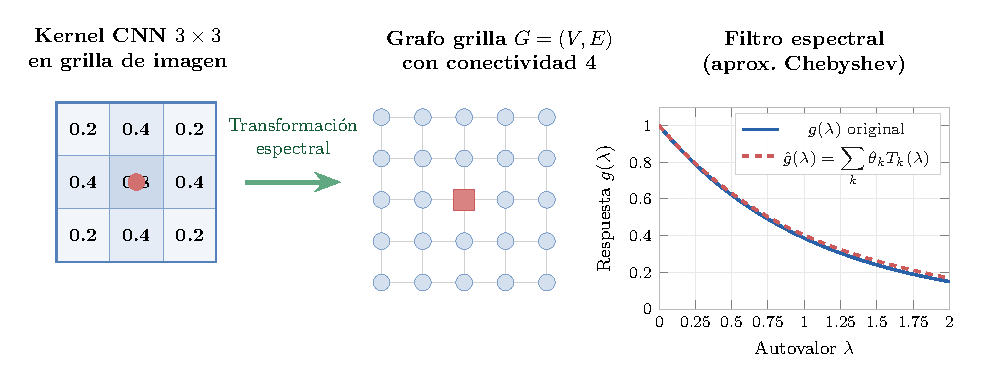
\includegraphics[width=0.95\textwidth]{images/cnn_to_spectral_graph}
	\caption[Transformation of a CNN kernel to its spectral representation on a grid graph]{Transformation of a CNN kernel to its spectral representation on a grid graph. Left: $3 \times 3$ kernel applied over an image grid with values proportional to the intensity. Center: representation of the same domain as a graph with 4-connectivity. Right: spectral filter $g(\lambda)$ and its approximation through Chebyshev polynomials $\hat{g}(\lambda) = \sum_k \theta_k T_k(\lambda)$.}
	\label{fig:cnn_to_spectral_graph}
\end{figure}

The next section will begin with group convolutions, where the regular grid structure is generalized to more complex homogeneous spaces, extending the unifying CNN-GNN framework towards richer geometric transformations.
